\documentclass[11pt]{article}

\usepackage[hyphens]{url}

\usepackage{hyperref}
\hypersetup
{
    breaklinks = true,
    allcolors = black,
    linktoc = all
}

\usepackage{graphicx}

\usepackage{multicol}
\setlength{\columnseprule}{0.4pt}

\usepackage{listings}

\usepackage[english]{babel}
\usepackage[utf8]{inputenc}
\usepackage{fancyhdr}
\pagestyle{fancy}
\fancyhf{}
\rhead{James Burton}
\lhead{ID: 4251529}
\fancyfoot[C]{\thepage}

\usepackage{titling}
\title
{ 
    G53IDS - Interim Report \\
    \hfill \break
    \large Embedded Domain Specific Language for \\
    Describing Recipes in Haskell
}

\setlength{\droptitle}{-10em}

\author{James Burton - 4251529 - psyjb6}

\begin{document}
    \maketitle
    \newpage

    \tableofcontents
    \newpage

    \section{Introduction}
    Consider the following recipe to make a cup of tea:

    \begin{tt}
    \small
    \begin{lstlisting}
    - Boil some water
    - Pour over a teabag
    - Wait for 3 minutes
    - Remove the teabag
    - Add milk (optional)
    \end{lstlisting}
    \end{tt}

    This is a very simple but useful recipe that many people
    will perform, in some cases, many times a day over their lives.
    What we can realise by looking at this recipe is that it actually
    consists of many smaller recipes, such as boiling water and
    combining tea with milk, performed in a certain order. This
    raises the question, to what extent does the order matter and
    to what extent can we rearrange things in order to make the recipe
    more efficient? No doubt you have done this, maybe subconsciously,
    while cooking at home. Furthermore which steps can be done
    concurrently in the event that multiple people are cooking e.g.
    in a professional kitchen with a full brigade? \\

    Perhaps closer to computer science, we could also ask, how could
    we instruct a robot to do this? After doing some research on
    robotic chefs it appears that not a huge number exist.
    There is one home cooking robot \cite{robot} which uses motion
    capture in order to learn recipes. In my opinion this is rather
    restrictive. It presumes that the human performs the recipe in
    the optimal manner and it would be very difficult to model
    a brigade system in this way. In reality there is a limited set
    of fundamental actions that one becomes able to perform when
    learning to cook. Recipes can then be performed using a sequence
    of these actions. Representing recipes like this would allow us
    to take a robot programmed to perform each of the fundamental
    actions and tell it how to cook literally anything. \\

    So we've established that if we can structure recipes in a more
    formal way then we will have a great amount of freedom in terms
    of how we process them whether it be optimisation for a human
    chef or full on automation. My contributions / planned contributions
    to this are the following:

    \begin{itemize}
        \item Define a set of combinators as an EDSL in Haskell and show that
        they can be used to describe a wide variety of recipes (Section 2).

        \item The combinators describe a recipe but we then need to know
        how to execute a recipe as a sequence of the fundamental actions
        mentioned above. Fortunately, as described above, recipes are just
        a combination of simpler recipes meaning that we can recursively
        define the actions necessary to perform complex recipes as long
        as we have manually defined which action are required for each
        combinator (Section 3).

        \item We now have a way to describe recipes and a way to show the
        sequence of actions to complete a recipe but now we need to apply
        them to something. Using the operational semantics of recipes
        we can optimise and schedule recipes for a given kitchen system.
        We can then express this in several ways including printing steps,
        drawing the cooking process as a graph or simulating the recipe
        within the given kitchen setup (Section 4).

        \item It may also be useful to provide an intermediate language
        between informal English and our combinators, some sort of markup
        language, that can then be parsed in.
    \end{itemize}

    \section{Describing Recipes}
    In this section I shall outline the EDSL for describing recipes.
    The EDSL is implemented in the functional programming language
    called Haskell which has been used for many EDSLs in the past \cite{hudak}.
    Michael Snoyman, creator of Yesod (a Haskell Web Framework), stated
    many advantages of using Haskell for EDSLs among which were that
    the type system helps catch mistakes and Haskell allows us to
    overload almost any syntax \cite{snoyman}.

    \subsection{A Cup of Tea}
    Consider our cup of tea example from earlier. We can start by
    defining all of our ingredients:

    \begin{tt}
    \small
    \begin{lstlisting}
        milk, teabag, water :: Recipe
        milk = Ingredient "milk"
        teabag = Ingredient "teabag"
        water = Ingredient "water"
    \end{lstlisting}
    \end{tt}

    The next step is to start describing what we want to transform
    those ingredients into for example:

    \begin{tt}
    \small
    \begin{lstlisting}
        boilingWater, blackTea :: Recipe
        boilingWater = heat 100 water
        blackTea = (teabag >< boilingWater) >>> Wait 5
    \end{lstlisting}
    \end{tt}

    We've introduced three things here. \texttt{heat} is simply
    a function meaning heat the given recipe to the given temperature.
    \texttt{><} is our combine operator and simply means mix the
    given recipes together. Finally \texttt{>>>} is our sequencing
    operator meaning do the first recipe then the second. The types
    for these are as follows: 
    
    \begin{tt}
    \small
    \begin{lstlisting}
        heat :: Temperature -> Recipe -> Recipe
        (><) :: Recipe -> Recipe -> Recipe
        (>>>) :: Recipe -> Recipe -> Recipe
    \end{lstlisting}
    \end{tt}

    We can now use the above to define our cup of tea recipe as follows:

    \begin{tt}
    \small
    \begin{lstlisting}
        cupOfTea :: Recipe
        cupOfTea = blackTea >< milk
    \end{lstlisting}
    \end{tt}

    Now you may notice that we haven't mentioned preparation of ingredients,
    for example measuring how much of them to use. While experimenting with
    the basic representation of a recipe and the different ways to interpret
    it we thought it would be beneficial to keep the combinators as simple
    and abstract as possible. This means that, for now, we will be describing
    recipes "cooking show" style where we presume everything is conveniently
    measured and prepared in a bowl next to the chef.

    \subsection{Currying - But Not What You Think}
    In this section I shall introduce the full set of combinators we are
    currently working with and proceed to build up a more complex recipe.

    \begin{figure}
        \centering
            \begin{multicols}{2}
                \raggedright
                \footnotesize
                \texttt{ingredient :: String -> Recipe} \\
                The recipe \texttt{(ingredient s)} simply represents an ingredient
                with the name s.

                \texttt{heat :: Temperature -> Recipe -> Recipe} \\
                \texttt{heat t r} means to heat the recipe r to the temperature t.

                \texttt{wait :: Time -> Recipe} \\
                \texttt{wait t} simply means do nothing for t amount of time.
                The decision to for \texttt{wait} to not include a recipe as
                an argument was very deliberate and will be discussed later
                in this subsection.

                \texttt{(><) :: Recipe -> Recipe -> Recipe} \\
                The recipe \texttt{r1 >< r2} is the combination of r1 and r2.
                The details of the method you use to combine the recipes are
                not yet captured.

                \texttt{(>>>) :: Recipe -> Recipe -> Recipe} \\
                \texttt{r1 >>> r2} represents the sequence of r1 and r2 i.e.
                perform recipe r1 followed by recipe r2.
            \end{multicols}
        \caption{Combinators for defining recipes}
    \end{figure}

    For the sake of conciseness I shalln't bother listing all the ingredient
    declarations here as they are relatively straightforward. \\

    We could just create a complex recipe outright however, this would be rather
    verbose and is likely to repeat a lot of code which somewhat goes against
    the core principles of DSLs and Haskell. Therefore we shall begin by defining
    some extra combinators made from our fundamental combinators. \\

    Marinating is a frequently used recipe so let's write a function for it:
    \begin{tt}
    \small
    \begin{lstlisting}
    marinate :: Recipe -> [Recipe] -> Recipe
    marinate r' (r:rs) = r' >< marinade
        where marinade = foldr (><) r rs
    \end{lstlisting}
    \end{tt}
    \texttt{marinate r' rs} means marinate \texttt{r'} in a marinade composed
    of the list of recipes \texttt{rs}. \\

    Due to the compositional nature of our combinators it is easy to create new
    ones like \texttt{marinate} thus allowing us to avoid repeating common
    sequences of recipes. There is no need to adjust any of our functions that
    work on recipes to work with \texttt{marinate} because it's just a combination
    of the combinators we already support. \\

    A huge number of recipes start by heating olive oil in a pan then adding something.
    We define the following combinator for this:
    \begin{tt}
    \small
    \begin{lstlisting}
    preheatOil :: Temeperature -> Recipe -> Recipe
    preheatOil t r = oil >< r
        where oil = heat t oliveOil
    \end{lstlisting}
    \end{tt}
    That is \texttt{preheatOil Medium onion} means heat some olive oil on medium heat
    then add some onion. \\

    I'm now going to explain the reasoning behind \texttt{wait} not taking a recipe as
    an argument. What this allows us to do is use \texttt{wait} in multiple ways.
    \texttt{wait t >< r} means perform recipe r for t amount of time whereas
    \texttt{r >>> wait t} means perform recipe r then wait for t. Using this we
    can define another combinator to allow us to heat a recipe at a given temperature
    but also for a certain time:
    \begin{tt}
    \small
    \begin{lstlisting}
    heatFor :: Temperature -> Recipe -> Time -> Recipe
    heatFor temp r time = (heat temp r) >< (wait time)
    \end{lstlisting}
    \end{tt}

    So let's get to that more complex recipe I mentioned earlier, Chicken Jalfrezi!
    \begin{tt}
    \small
    \begin{lstlisting}
    spicedChicken :: Recipe
    spicedChicken = marinate chicken [cumin, coriander, turmeric]

    chickenAndPeppers :: Recipe
    chickenAndPeppers = heatFor Medium (cookedChicken >< redPeppers) 10
        where cookedChicken = heatFor Medium spicedChicken 10

    jalfreziSauce :: Recipe
    jalfreziSauce = heatFor Medium (sauceBase >< spices) 10
        where
            onionMix = onion >< garlic >< greenChilli
            cookedOnions = heatFor Medium (preheatOil Medium onionMix) 5
            spices = cumin >< coriander >< turmeric >< garamMasala
            sauceBase = cookedOnions >< water >< tinnedTomatoes >< spices

    chickenJalfrezi :: Recipe
    chickenJalfrezi = heatFor Medium chickenJalfrezi' 5
        where chickenJalfrezi' = chickenAndPeppers >< jalfreziSauce >< cherryTomatoes
    \end{lstlisting}
    \end{tt}
    And there we have it. Quite a large recipe expressed formally with
    multiple reusable components. As the project continues, the set of
    combinators will continue to evolve as we run in to issues. Some of
    these issues have already been discovered and will be discussed later
    (Sections 3.3 & 5.2).

    \subsection{Conditionals}

    Mention wait combination.

    (Heat Medium oliveOil) >< onion, are we still heating the onion!?

    \subsection{Moving Forward}
    At the time of writing this interim report, the combinators we
    have are decent but not perfect. There are several crucial pieces
    of information not captured such as measurements and, as mentioned
    above, conditionals and optional recipes are not yet implemented. \\

    Now that we have a more detailed idea of the components of the project,
    we can move towards implementing them. That will naturally provide
    an opportunity to scrutinise the set of combinators we are working
    with by analysing any issues we run into.

    \section{Executing a Recipe}
    \begin{figure}[ht]
        \centering
            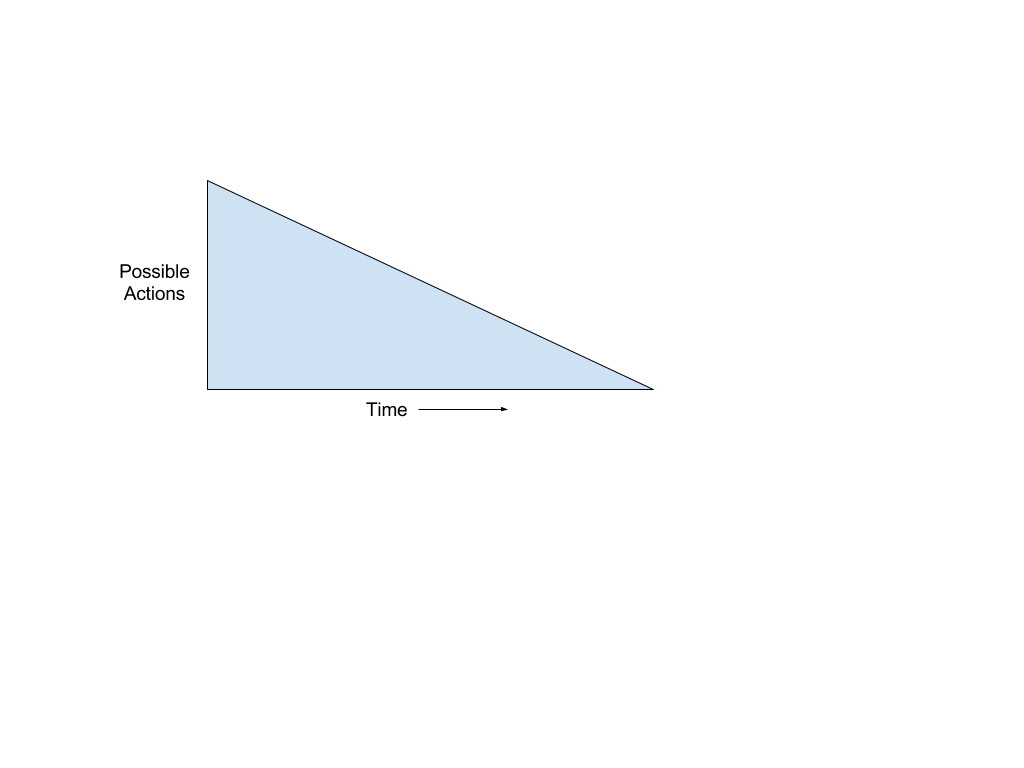
\includegraphics[width=\textwidth,keepaspectratio]{actions_time.png}
        \caption{Number of possible actions over time.}
    \end{figure}

    \begin{figure}[ht]
        \centering
            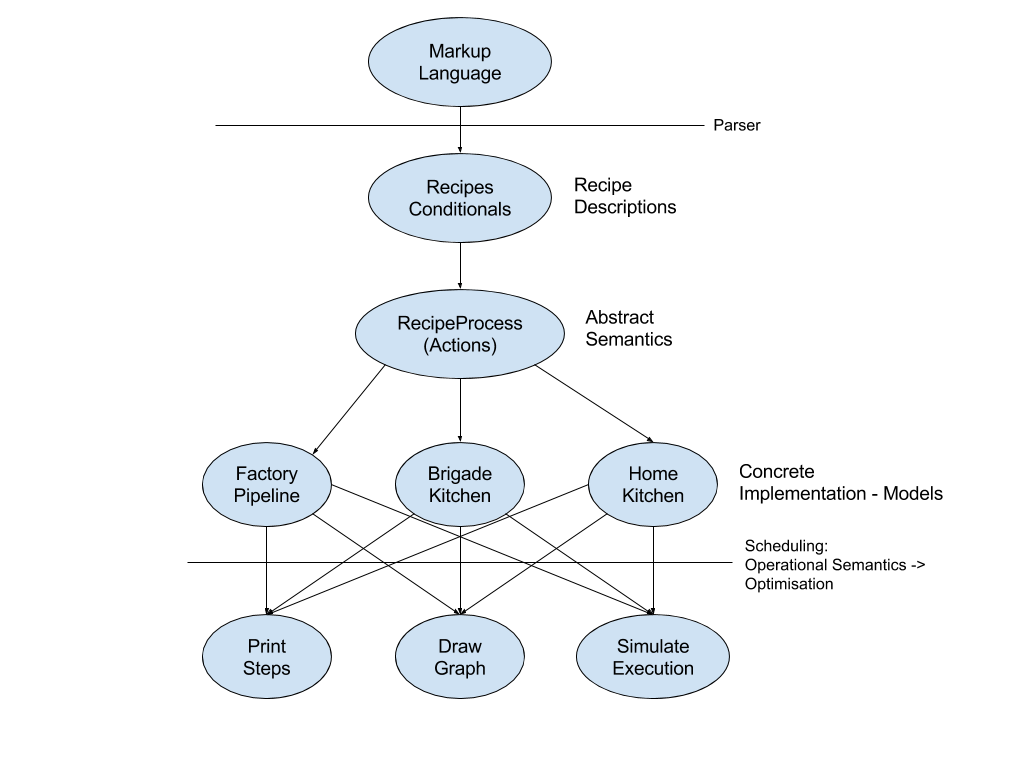
\includegraphics[width=\textwidth,keepaspectratio]{recipe_flow.png}
        \caption{Components of the recipe system.}
    \end{figure}

    
    \section{Implementation}

    \section{Progress}
    This project shall use the scrum development methodology. With the
    gaps between supervisor meetings acting as the sprints. The scrum
    methodology seems most appropriate for this project as it is naturally
    very flexibly and doesn't require a huge amount of detailed planning
    in advance. This suits the research nature of the project as it is
    impossible to precisely state what will be done and when. Each sprint
    offers an opporuntity to re-prioritise and alter tasks based upon
    the progress and findings of the previous sprint.
    \subsection{Project Management}
    \subsection{Contributions and Reflections}

    \section{Related Work}

    \newpage
    \begin{thebibliography}{0}

        \bibitem{robot}
        The Guardian. 2015. \textit{Future of food: how we cook}.
        \url{https://www.theguardian.com/technology/2015/sep/13/future-of-food-how-we-cook}

        \bibitem{hudak}
        Paul Hudak. Domain Specific Languages. Department of Computer
        Science, Yale University, December 15, 1997.

        \bibitem{snoyman}
        Michael Snoynman. O'Reilly Webcast: Designing Domain Specific
        Languages with Haskell. January 4, 2013.
        \url{https://www.youtube.com/watch?v=8k_SU1t50M8}

        \bibitem{contracts}
        Simon Peyton Jones, Microsoft Research, Cambridge.
        Jean-Marc Eber, LexiFi Technologies, Paris. Julian Seward,
        University of Glasgow. Composing contracts: an adventure in
        financial engineering. August 17, 2000.


    \end{thebibliography}   
     
\end{document}